\documentclass{beamer}
\beamertemplatenavigationsymbolsempty
\usecolortheme{beaver}
\setbeamertemplate{blocks}[rounded=true, shadow=true]
\setbeamertemplate{footline}[page number]
%
\usepackage[utf8]{inputenc}
\usepackage[english,russian]{babel}
\usepackage{amssymb,amsfonts,amsmath,mathtext}
\usepackage{subfig}
\usepackage[all]{xy} % xy package for diagrams
\usepackage{array}
\usepackage{multicol} % many columns in slide
\usepackage{hyperref} % urls
\usepackage{hhline} %tables
\usepackage{comment} %comments
% Your figures are here:
\graphicspath{ {../figures/} }

%----------------------------------------------------------------------------------------------------------

\title[\hbox to 56mm{Дистилляция знаний в глубоких сетях с применением методов выравнивания структур моделей}]{Дистилляция знаний в глубоких сетях с применением методов выравнивания структур моделей}
\author[М.\,С.~Олейник]{Михаил Сергеевич Олейник}
\institute{Московский физико-технический институт}
\date{\footnotesize
\par\smallskip\emph{Научный руководитель:} О. Ю. Бахтеев
\par\bigskip\small 2023}

%----------------------------------------------------------------------------------------------------------
\begin{document}
%----------------------------------------------------------------------------------------------------------

\begin{frame}

    \thispagestyle{empty}
    \maketitle

\end{frame}

%-----------------------------------------------------------------------------------------------------

\begin{frame}{Цели исследования}

    \textbf{Проблема}: сложно проводить дистилляцию, если ученик и учитель имеют сильно отличающиеся архитектуры.
    А если не сложно, то это дистилляция по Хинтону.

    \bigskip

    \textbf{Цель}: предложить метод дистилляции, который будет работать для разных архитектур и с разным количеством слоёв.

\end{frame}

%-----------------------------------------------------------------------------------------------------

\begin{frame}{Литература}
    \begin{itemize}
        \item Sungsoo Ahn et al. "Variational information distillation for knowledge transfer"
        \item Nikolaos Passalis, Maria Tzelepi, and Anastasios Tefas. "Heterogeneous knowledge distillation using
              information flow modeling"
        \item M Gorpinich, O Yu Bakhteev, and VV Strijov. "Gradient methods for optimizing metaparameters in the
              knowledge distillation problem"
    \end{itemize}
\end{frame}

%----------------------------------------------------------------------------------------------------------

\begin{frame}{Постановка задачи}
    Дана выборка для задачи классификации на $K$ классов:

    $$\mathfrak{D}  = \{(\bold{x}_i, y_i)\}_{i=1}^{m},\; \bold{x}_i \in \mathbb{R}^n,\; y_i \in \mathbb{Y}  = \{1, \dots, K\},$$

    $$\mathfrak{D} = \mathfrak{D}_\text{train} \bigsqcup \mathfrak{D}_\text{test}.$$

    Обозначим:
    \begin{itemize}
        \item $\bold{f}$ --- модель учителя, обученная на $\mathfrak{D}_\text{train}$
        \item $\bold{g}$ --- модель ученика, которую предстоит обучить
        \item $T$ --- количество слоев в учителе
        \item $S$ --- количество слоев в ученике
        \item $t_i$ --- активации в $i$-м слое учителя
        \item $s_i$ --- активации в $i$-м слое ученика
    \end{itemize}
\end{frame}


%----------------------------------------------------------------------------------------------------------

\begin{frame}{Постановка задачи}
    Функцию потерь ученика представим как:
    $$
        \mathcal{L} = \beta \mathcal{L}_\text{task} - (1 - \beta){\sum_{i, j=1}^{T, S}\lambda_{i, j}I(t_{i}, s_{j})},
    $$
    Где:
    \begin{itemize}
        \item $\mathcal{L}_\text{task}$ --- функция потерь для решения задачи классификации (кросс-энтропия),
        \item $I(t_{i}, s_{j})$ --- взаимная информация,
        \item $\beta$ и $\lambda_{i, j}$ --- гиперпараметры.
    \end{itemize}
\end{frame}

%----------------------------------------------------------------------------------------------------------

\begin{frame}{Взаимная информация}
    Метод вариации нижней границы:
    \begin{equation}
        I(t, s) = H(t) - H(t|s) \geq  H(t) + E_{t,s}[\log{q(t|s)}].
    \end{equation}
    Вариационное распределение:
    \begin{multline}
        -\log{q(t|s)} = -\sum_{c=1}^{C}  \sum_{h=1}^{H} \sum_{w=1}^{W} \log{q(t_{c,h,w}|s)} = \\
        = \sum_{c=1}^{C}  \sum_{h=1}^{H} \sum_{w=1}^{W} \log{\sigma_c} + \frac{(t_{c,h,w} - \mu_{c,h,w}(s))^2}{2\sigma_c^2} + constant.
    \end{multline}
    Обучаемые параметры:
    $$\sigma^2_c = \log{(1 + e^{\alpha_c})} + \epsilon$$
    $$\mu_{c,h,w}(s) = \mu(s)_{c,h,w}$$
\end{frame}

%-----------------------------------------------------------------------------------------------------

\begin{frame}{Схема метода}

    \begin{columns}[c]
        \column{0.4\textwidth}
        \begin{figure}
            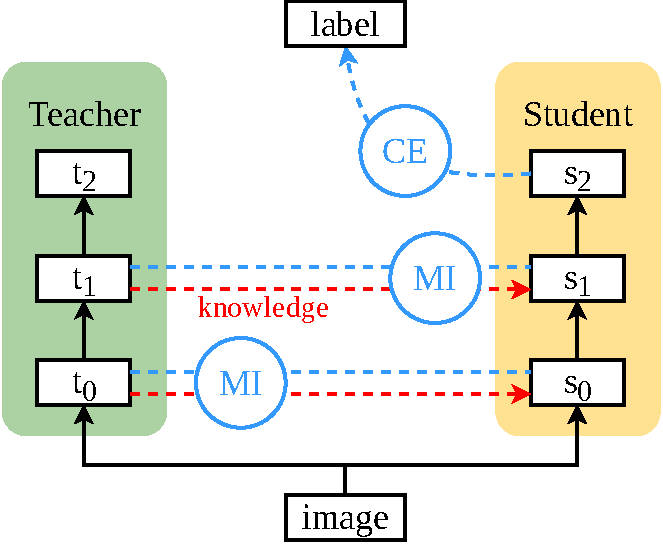
\includegraphics[width=1.0\textwidth]{ahn_diagram.pdf}
            \caption{Базовый метод \footnote{Sungsoo Ahn et al. "Variational information distillation for knowledge transfer"}}
        \end{figure}

        \column{0.4\textwidth}
        \begin{figure}
            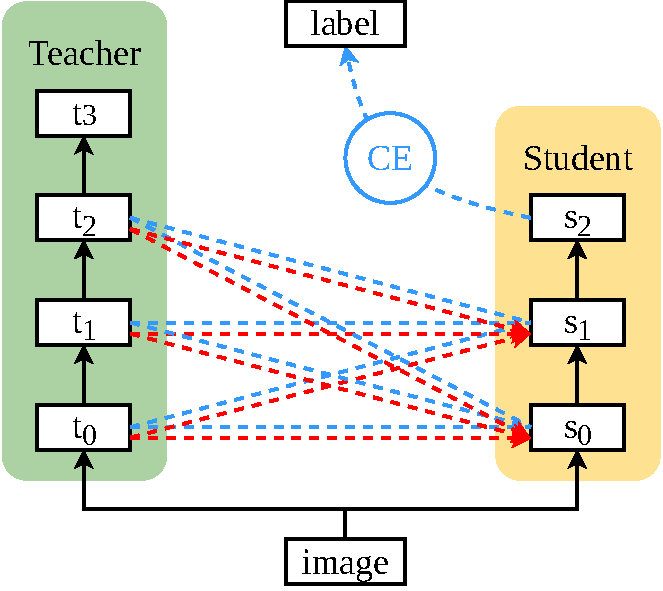
\includegraphics[width=1.0\textwidth]{our_diagram.pdf}
            \caption{Предлагаемый метод}
        \end{figure}
    \end{columns}

    \begin{equation}
        \mathcal{L} = \beta \mathcal{L}_\text{CE} - (1 - \beta){\sum_{i, j=1}^{T, S}\lambda_{i, j}I(t_{i}, s_{j})}
    \end{equation}


\end{frame}


%----------------------------------------------------------------------------------------------------------

\begin{frame}{Вычислительный эксперимент}
    \begin{columns}[c]
        \column{0.4\textwidth}
        Датасеты:
        \begin{itemize}
            \item CIFAR10
        \end{itemize}
        Модели:
        \begin{itemize}
            \item ConvVeryTiny
            \item ConvTiny
            \item ResNet10
            \item ResNet18
        \end{itemize}
        Метрики:
        \begin{itemize}
            \item accuracy
        \end{itemize}
        \column{0.45\textwidth}
        \begin{figure}
            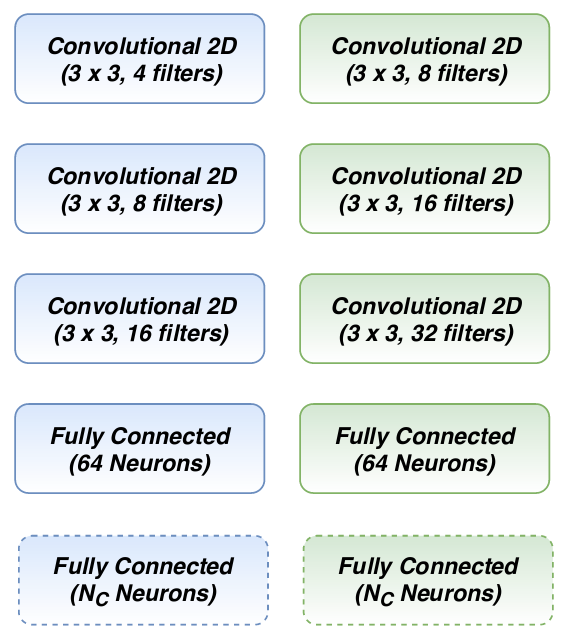
\includegraphics[width=1.0\textwidth]{conv_scheme.png}
            \caption{Схема моделей ConvVeryTiny и ConvTiny}
        \end{figure}
    \end{columns}
\end{frame}

%----------------------------------------------------------------------------------------------------------

\begin{frame}{Эксперимент 1}
    \begin{columns}[c]
        \column{0.4\textwidth}
        \textbf{Учитель}: ConvTiny.

        \textbf{Ученик}: ConvVeryTiny.


        \column{0.55\textwidth}
        \begin{figure}
            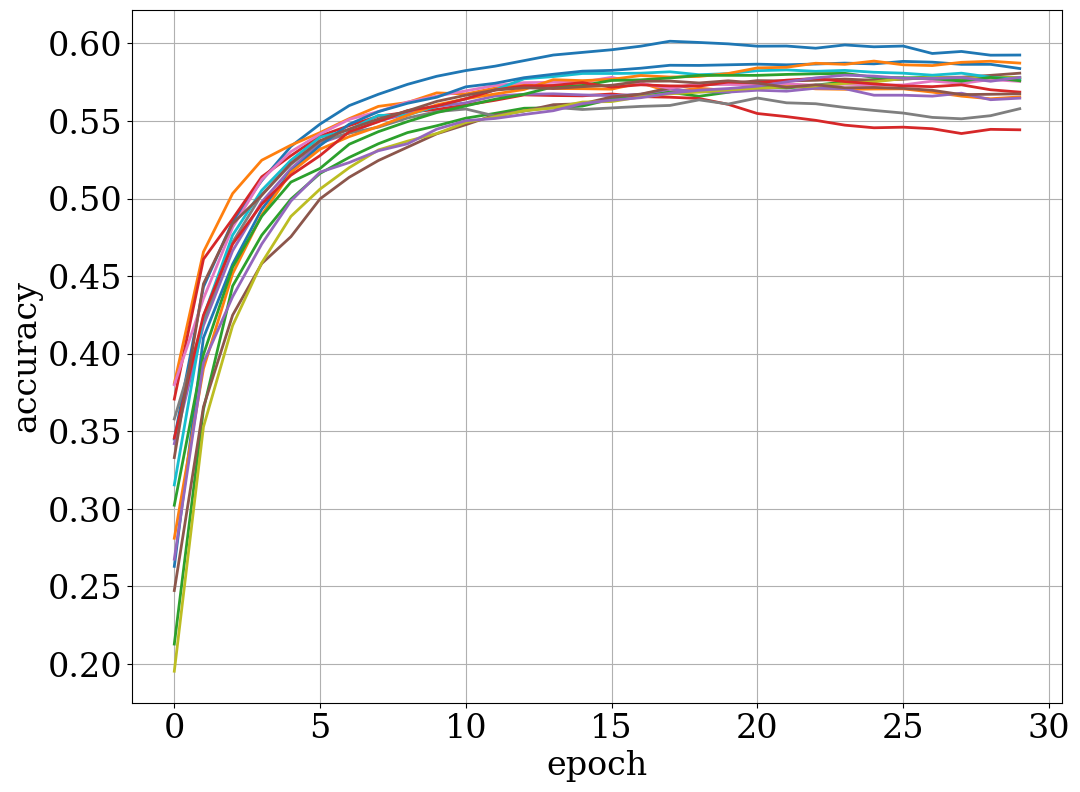
\includegraphics[width=1.0\textwidth]{distill_epoch_accuracy.png}
            \caption{Точность от эпохи при дистилляции каждый с каждым}
        \end{figure}
    \end{columns}

    \begin{table}[]
        \begin{tabular}{|l|l|l|l|l|}
            \hline
            Дистилляция & ---  & Хинтона & попарная  & каждый с каждым \\ \hline
            Учитель     & 0.58 & ---     & ---       & ---             \\ \hline
            Ученик      & 0.54 & 0.56    & 0.58-0.59 & 0.58-0.59       \\ \hline
        \end{tabular}
        \caption{Сравнение качества моделей на тестовой выборке}
    \end{table}
\end{frame}

%----------------------------------------------------------------------------------------------------------

\begin{frame}{Эксперимент 1}
    \begin{figure}[H]
        \begin{minipage}[h]{0.35\linewidth}
            \center{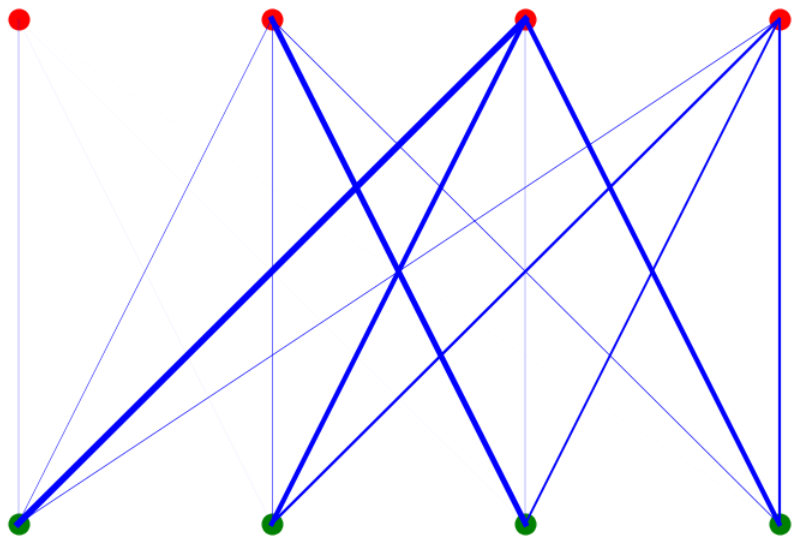
\includegraphics[width=1\linewidth]{connections_1}} a) \\
        \end{minipage}
        \hfill
        \begin{minipage}[h]{0.35\linewidth}
            \center{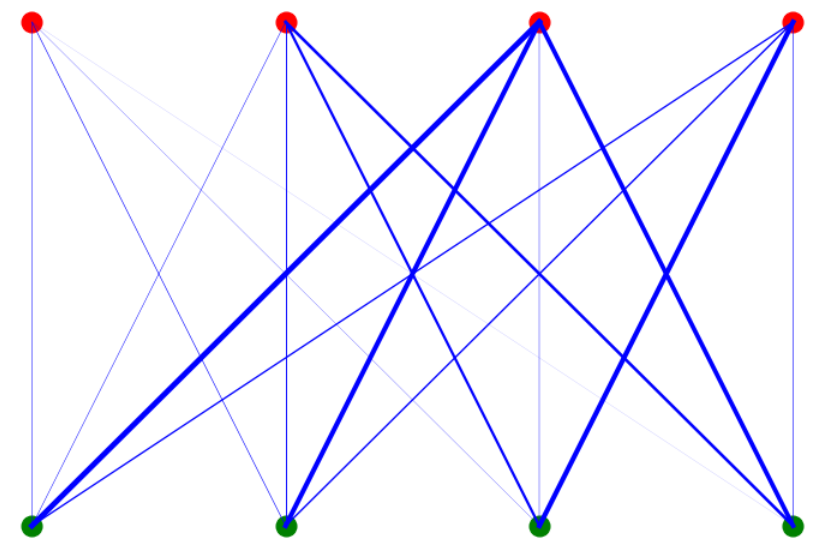
\includegraphics[width=1\linewidth]{connections_2}} b) \\
        \end{minipage}
        \vfill
        \begin{minipage}[h]{0.35\linewidth}
            \center{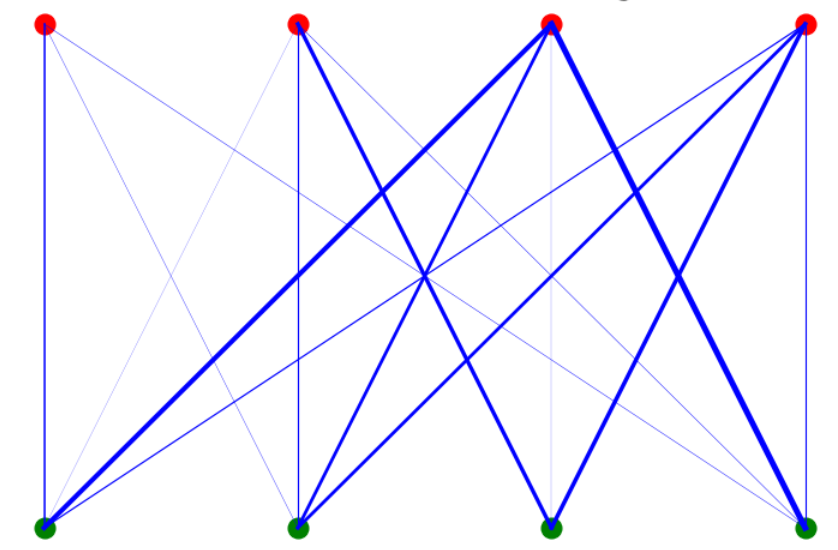
\includegraphics[width=1\linewidth]{connections_3}} c) \\
        \end{minipage}
        \hfill
        \begin{minipage}[h]{0.35\linewidth}
            \center{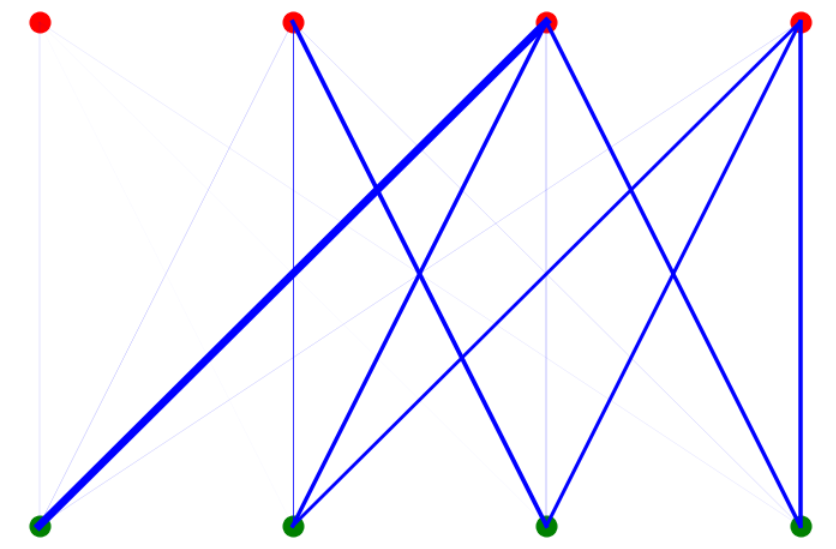
\includegraphics[width=1\linewidth]{connections_4}} d) \\
        \end{minipage}
        \caption{Иллюстрация коэффициентов у четырех лучших моделей по качеству. Зелёные точки --- слои ученика, красные --- слои учителя. Чем толще линия, тем больше коэффициент у соответствующей связи.}
    \end{figure}
\end{frame}

%----------------------------------------------------------------------------------------------------------

\begin{frame}{Эксперимент 2}
    \begin{columns}[c]
        \column{0.4\textwidth}
        \textbf{Учитель}: ResNet10.

        \textbf{Ученик}: ConvTiny.

        \column{0.55\textwidth}
        \begin{figure}
            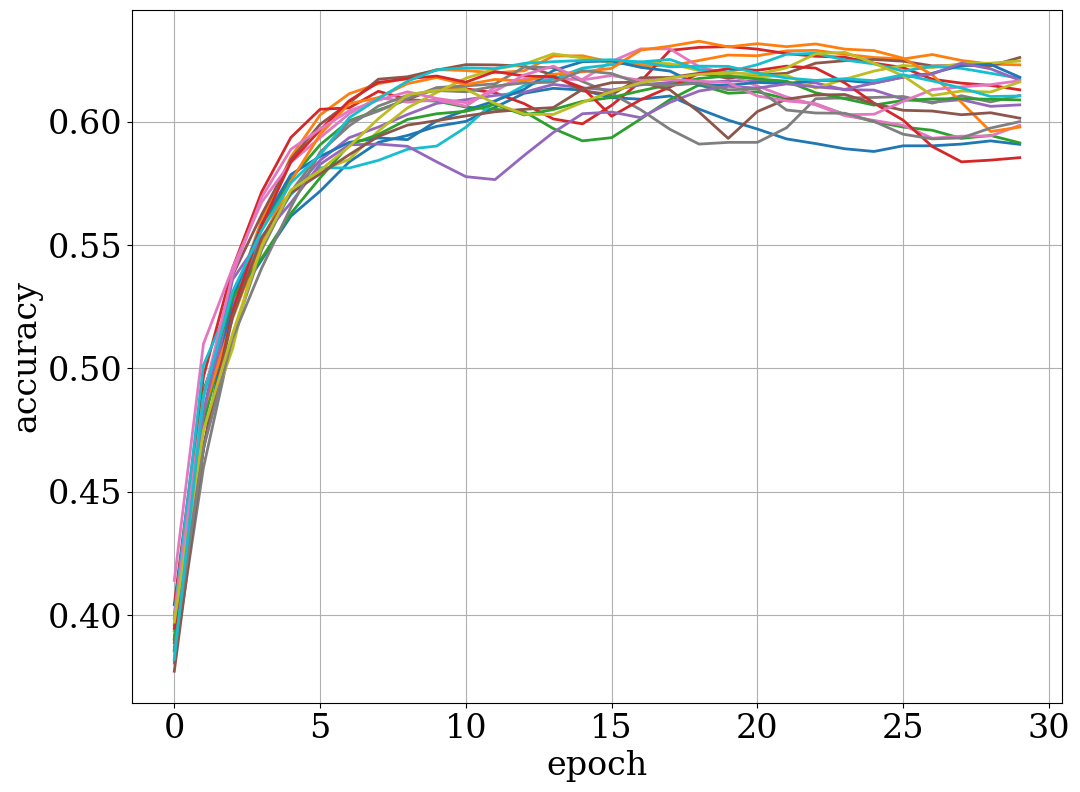
\includegraphics[width=1.0\textwidth]{resnet10_tiny.png}
            \caption{Точность от эпохи при дистилляции каждый с каждым}
        \end{figure}
    \end{columns}

    \begin{table}[h!]
        \centering
        \begin{tabular}{|l|l|l|l|}
            \hline
            Дистилляция & ---  & Хинтона & каждый с каждым \\ \hline
            Учитель     & 0.68 & ---     & ---             \\ \hline
            Ученик      & 0.58 & 0.60    & 0.63            \\ \hline
        \end{tabular}
        \caption{Качество моделей при дистилляции на тестовой выборке}
    \end{table}
\end{frame}

%----------------------------------------------------------------------------------------------------------

\begin{frame}{Эксперимент 2}
    \begin{figure}[H]
        \begin{minipage}[h]{0.35\linewidth}
            \center{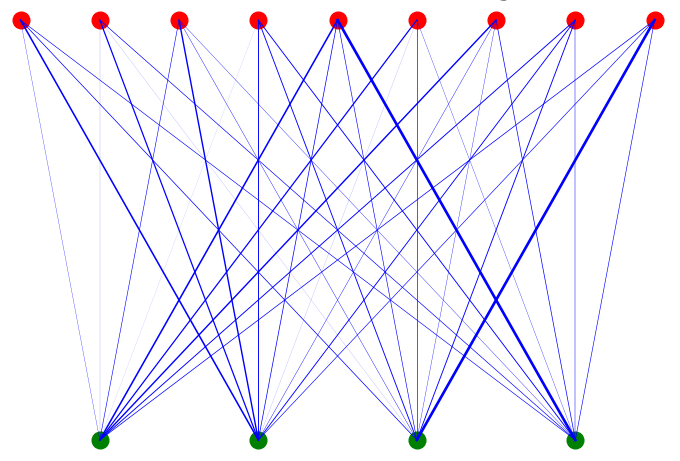
\includegraphics[width=1\linewidth]{r10_conn_1}} a) \\
        \end{minipage}
        \hfill
        \begin{minipage}[h]{0.35\linewidth}
            \center{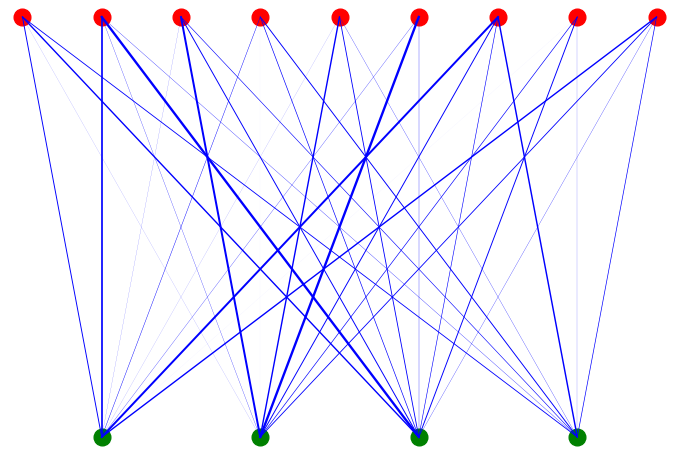
\includegraphics[width=1\linewidth]{r10_conn_2}} b) \\
        \end{minipage}
        \vfill
        \begin{minipage}[h]{0.35\linewidth}
            \center{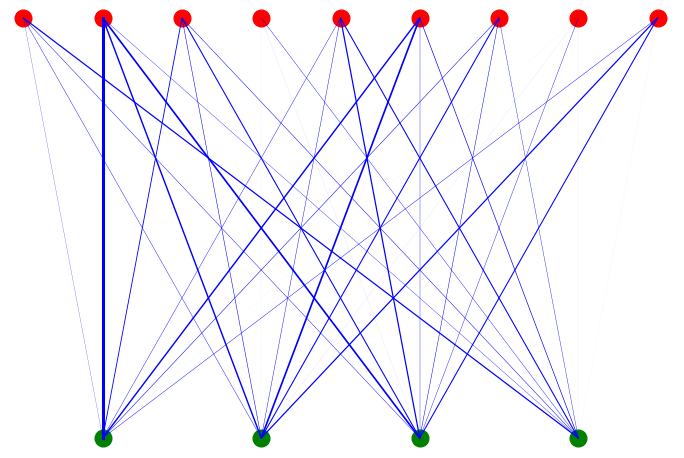
\includegraphics[width=1\linewidth]{r10_conn_3}} c) \\
        \end{minipage}
        \hfill
        \begin{minipage}[h]{0.35\linewidth}
            \center{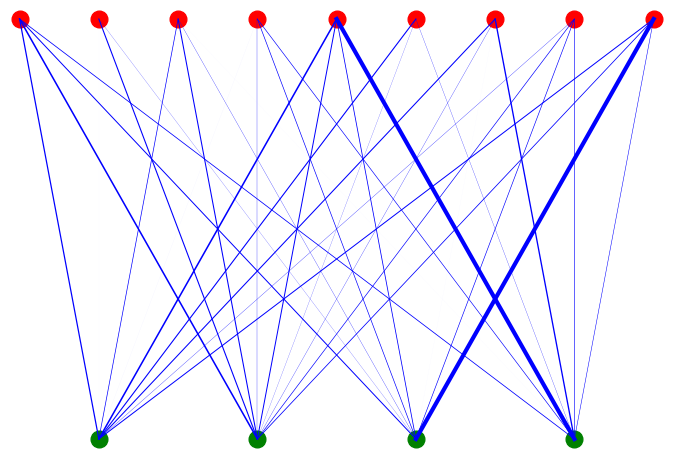
\includegraphics[width=1\linewidth]{r10_conn_4}} d) \\
        \end{minipage}
        \caption{Иллюстрация коэффициентов у четырех лучших моделей по качеству. Зелёные точки --- слои ученика, красные --- слои учителя. Чем толще линия, тем больше коэффициент у соответствующей связи.}
    \end{figure}
\end{frame}

%----------------------------------------------------------------------------------------------------------

\begin{frame}{Заключение}
    Был предложен метод дистилляции знаний, который можно применить к моделям с разным количеством слоев и/или разными архитектурами,
    который выдает большее качество, чем дистилляция Хинтона. Однако, к недостаткам данного подхода можно отнести большие требования по памяти и времени,
    если модель учителя и/или ученика имеет большое количество слоёв. В дальнейших планах стоит более тщательное изучение влияния связей между слоями на итоговый результат,
    что потенциально и может свести недостатки подхода к минимуму.
\end{frame}

%----------------------------------------------------------------------------------------------------------
\end{document}